% FluidWorld: Reaction-Diffusion Dynamics as a Predictive Substrate for World Models
% NeurIPS 2026 Submission
%
% Compile: pdflatex fluidworld.tex && bibtex fluidworld && pdflatex fluidworld.tex && pdflatex fluidworld.tex

\documentclass{article}

% NeurIPS 2026 style
\usepackage[final]{neurips_2025}

\usepackage[utf8]{inputenc}
\usepackage[T1]{fontenc}
\usepackage{hyperref}
\usepackage{url}
\usepackage{booktabs}
\usepackage{amsfonts}
\usepackage{amsmath}
\usepackage{amssymb}
\usepackage{nicefrac}
\usepackage{microtype}
\usepackage{graphicx}
\usepackage{subcaption}
\usepackage{algorithm}
\usepackage{algorithmic}
\usepackage{xcolor}
\usepackage{multirow}
\usepackage{wrapfig}

% Custom commands
\newcommand{\ie}{\textit{i.e.}}
\newcommand{\eg}{\textit{e.g.}}
\newcommand{\cf}{\textit{cf.}}
\newcommand{\etal}{\textit{et al.}}
\newcommand{\R}{\mathbb{R}}
\newcommand{\N}{\mathbb{N}}
\newcommand{\lapl}{\nabla^2}
\newcommand{\fluidworld}{\textsc{FluidWorld}}
\DeclareMathOperator{\softplus}{softplus}
\DeclareMathOperator{\sigmoid}{sigmoid}
\DeclareMathOperator{\gelu}{GELU}

\title{\fluidworld{}: Reaction-Diffusion Dynamics as a\\Predictive Substrate for World Models}

\author{
  Fabien Polly \\
  Independent Researcher \\
}

\begin{document}

\maketitle

% ============================================================================
\begin{abstract}
% ============================================================================
World models learn to predict future states of an environment, enabling planning and imagination. Current approaches rely on Transformer-based predictors operating in learned latent spaces, inheriting their $O(N^2)$ computational cost and lacking explicit spatial inductive biases. This paper asks a foundational question: \emph{is self-attention necessary for predictive world modeling, or can alternative computational substrates achieve comparable or superior results?} I introduce \fluidworld{}, a proof-of-concept world model whose predictive dynamics are governed by \emph{partial differential equations} (PDEs) of reaction-diffusion type. Instead of using a separate neural network predictor, the PDE integration \emph{itself} produces the future state prediction. In a strictly parameter-matched three-way ablation on unconditional UCF-101 video prediction ($64\!\times\!64$, $\sim$800K parameters, identical encoder, decoder, losses, and data), \fluidworld{} is compared against both a Transformer baseline (self-attention) and a ConvLSTM baseline (convolutional recurrence). While all three models converge to comparable single-step prediction loss, \fluidworld{} achieves $2\times$ lower reconstruction error, produces representations with 10--15\% higher spatial structure preservation and 18--25\% more effective dimensionality, and critically maintains coherent multi-step rollouts where both baselines degrade rapidly. All experiments were conducted on a single consumer-grade PC (Intel Core i5, NVIDIA RTX 4070 Ti), without any large-scale compute. These results establish that PDE-based dynamics -- which natively provide $O(N)$ spatial complexity, adaptive computation, and global spatial coherence through diffusion -- are a viable and parameter-efficient alternative to both attention and convolutional recurrence for world modeling.
\end{abstract}

% ============================================================================
\section{Introduction}
\label{sec:introduction}
% ============================================================================

Learning predictive models of the world -- commonly called \emph{world models} -- is a central challenge in artificial intelligence~\cite{lecun2022path,ha2018worldmodels}. A world model takes an observation $x_t$ and predicts the future state $x_{t+1}$ or its abstract representation, optionally conditioned on actions. Such models enable agents to plan by simulating the consequences of candidate actions before execution~\cite{hafner2023dreamerv3,schrittwieser2020muzero}.

The dominant paradigm uses \emph{Transformer}-based architectures~\cite{vaswani2017attention} as the predictive engine. This is a choice by default, not by principle. Joint Embedding Predictive Architecture (JEPA)~\cite{lecun2022path,assran2023ijepa,bardes2024vjepa} predicts latent representations rather than pixels, using Vision Transformers (ViT)~\cite{dosovitskiy2021vit} as both encoders and predictors. While powerful, this approach has fundamental limitations:

\begin{enumerate}
    \item \textbf{$O(N^2)$ spatial cost.} Self-attention over $N$ spatial tokens scales quadratically, limiting resolution.
    \item \textbf{No spatial inductive bias.} Transformers must \emph{learn} spatial propagation from data, consuming model capacity for what physics provides for free.
    \item \textbf{Fixed computation.} Every prediction costs the same, regardless of complexity.
    \item \textbf{No persistent state.} Each prediction is independent; temporal context requires explicit memory mechanisms.
\end{enumerate}

This paper is an \emph{architectural proof-of-concept}. I do not aim to beat state-of-the-art world models that use orders of magnitude more parameters and compute. Instead, I ask whether attention is strictly necessary for predictive world modeling, or whether an alternative computational substrate -- one grounded in physics rather than combinatorics -- can match or exceed Transformers at equal parameter budget.

Furthermore, while world models are ultimately designed for action-conditioned planning, their foundational prerequisite is \emph{stable temporal prediction}. To rigorously isolate and evaluate the predictive capacity of the PDE substrate, the experiments in this paper focus entirely on unconditional video prediction. Although the \fluidworld{} architecture natively supports action conditioning via additive forcing terms in the PDE, evaluating differentiable planning through the PDE dynamics is left as a critical next step for future work.

I propose \fluidworld{}, a world model that replaces attention-based prediction with \emph{reaction-diffusion partial differential equations} (PDEs). The key insight is simple: the PDE integration itself constitutes the prediction. An observation is encoded into a spatial feature map, and PDE dynamics -- diffusion for spatial propagation, learned reaction terms for nonlinear transformation, and optional forcing terms for action conditioning -- evolve the latent state toward the predicted future. This formulation inherits the physics of reaction-diffusion systems: $O(N)$ local computation, adaptive convergence, and continuous temporal dynamics.

The contributions of this work are:
\begin{enumerate}
    \item \textbf{PDE-native world model.} I demonstrate that reaction-diffusion dynamics can serve as the predictive engine of a world model, replacing self-attention entirely (\S\ref{sec:method}).
    \item \textbf{BeliefField.} A persistent latent state that accumulates temporal context through PDE evolution, with biologically-inspired mechanisms (Hebbian diffusion, synaptic fatigue, lateral inhibition) that improve representational diversity (\S\ref{sec:belief}).
    \item \textbf{Three-way parameter-controlled ablation.} I compare \fluidworld{} against both a Transformer baseline (self-attention) and a ConvLSTM baseline (convolutional recurrence) at \emph{identical} parameter count ($\sim$800K), same encoder, same decoder, same losses, and same data, isolating the effect of the predictive substrate (\S\ref{sec:experiments}).
    \item \textbf{Efficiency and rollout analysis.} I characterize the $O(N)$ vs $O(N^2)$ scaling advantage, show that PDE dynamics produce richer spatial representations per parameter, and demonstrate superior multi-step rollout coherence compared to both baselines (\S\ref{sec:analysis}).
\end{enumerate}

% ============================================================================
\section{Related Work}
\label{sec:related}
% ============================================================================

\paragraph{World Models.}
Ha and Schmidhuber~\cite{ha2018worldmodels} introduced the concept of learned world models using VAE encoders and RNN-based dynamics. Dreamer~\cite{hafner2020dreamerv1,hafner2021dreamerv2,hafner2023dreamerv3} extended this with RSSM (Recurrent State-Space Models), achieving strong results in continuous control. MuZero~\cite{schrittwieser2020muzero} learns a world model for planning in discrete action spaces. IRIS~\cite{micheli2023iris} and TWM~\cite{robine2023twm} use Transformer-based world models with discrete latent spaces. All these approaches use standard neural network architectures (RNNs, Transformers, MLPs) as their predictive engine.

\paragraph{JEPA and Self-Supervised Prediction.}
LeCun~\cite{lecun2022path} proposed JEPA as a blueprint for autonomous intelligence, predicting in representation space rather than pixel space. I-JEPA~\cite{assran2023ijepa} and V-JEPA~\cite{bardes2024vjepa} validate this for images and video using ViT predictors. MC-JEPA~\cite{bardes2023mcjepa} separates motion and content. These works establish representation prediction as viable but retain Transformer predictors.

\paragraph{PDE-Inspired Neural Networks.}
Neural ODEs~\cite{chen2018neuralode} interpret residual networks as ODE discretizations. PDE-Net~\cite{long2018pdenet,long2019pdenet2} learns PDE coefficients for physical simulation. Neural Operators~\cite{li2021fno} learn solution operators for PDEs. Reaction-diffusion networks have been explored for image segmentation~\cite{luo2023rdnet} and graph processing~\cite{chamberlain2021grand}. This work differs fundamentally: I use PDEs not to \emph{simulate} physical systems, but as the \emph{computational substrate} of a learned world model.

\paragraph{Video Prediction.}
Convolutional recurrent architectures have a long history in video prediction. ConvLSTM~\cite{shi2015convlstm} introduced convolutional gates for spatiotemporal sequence modeling. PredRNN~\cite{wang2017predrnn,wang2022predrnnv2} proposed spatiotemporal LSTM units with zigzag memory flow. SimVP~\cite{gao2022simvp} showed that simple convolutional architectures can match recurrent models on standard benchmarks. These approaches provide a natural middle ground between purely spatial (ConvNet) and purely global (Transformer) processing, and represent important baselines for any spatial prediction architecture.

\paragraph{Efficient Alternatives to Attention.}
Linear attention~\cite{katharopoulos2020linear}, state-space models (S4, Mamba)~\cite{gu2022s4,gu2024mamba}, and local attention patterns~\cite{liu2021swin} reduce the $O(N^2)$ cost. My approach is orthogonal: instead of making attention cheaper, I replace it entirely with PDE dynamics that are $O(N)$ by construction.

% ============================================================================
\section{From Language to World Models: The Fluid Architecture Lineage}
\label{sec:lineage}
% ============================================================================

\fluidworld{} is the third iteration of a research program exploring reaction-diffusion PDEs as a general-purpose computational substrate, progressively replacing attention in different modalities:

\paragraph{FluidLM (2024): Language.} The initial exploration replaced self-attention with reaction-diffusion dynamics in a language model. A 1D Laplacian operator propagated information along the token sequence, with learned reaction terms providing nonlinear mixing. This proof-of-concept demonstrated that PDE dynamics could process sequential data, though at a performance gap compared to standard Transformers for language tasks.

\paragraph{FluidVLA (2025): Vision and Robotics.} The architecture was adapted to 2D spatial data using \texttt{FluidLayer2D} with a 2D Laplacian operator. FluidVLA achieved competitive results in image classification and real-time robotic control (40\,ms inference on an NVIDIA RTX 4070), demonstrating that PDE-based processing scales to visual perception tasks. Key innovations at this stage included multi-scale dilated Laplacians (dilations $\{1, 4, 16\}$), adaptive early stopping based on convergence monitoring, and \texttt{MemoryPump} for $O(1)$ global context. FluidVLA was further extended to \texttt{FluidLayer3D} for volumetric medical imaging (CT/MRI segmentation), where the $O(N)$ scaling advantage over attention became particularly relevant for processing high-resolution 3D volumes.

\paragraph{FluidWorld (2026): World Models.} This work extends the PDE substrate from perception to prediction. The core innovation is that the same reaction-diffusion equation used for spatial encoding also serves as the temporal prediction mechanism, via the BeliefField (\S\ref{sec:belief}). Biologically-inspired mechanisms (synaptic fatigue, lateral inhibition, Hebbian diffusion) were added to improve representational diversity in the temporal prediction setting, where channel collapse is a greater risk than in single-frame classification.

This progression demonstrates the generality of the PDE substrate across modalities (1D sequences, 2D images, 3D volumes, temporal prediction), with each iteration refining the core equation while maintaining $O(N)$ complexity and adaptive computation.

% ============================================================================
\section{Method}
\label{sec:method}
% ============================================================================

\subsection{Overview}

\fluidworld{} processes video frames through three stages (Figure~\ref{fig:architecture}):
\begin{enumerate}
    \item \textbf{Encode}: A frame $x_t \in \R^{C \times H \times W}$ is mapped to spatial features $z_t \in \R^{d \times H_f \times W_f}$ via patch embedding followed by PDE-based processing layers.
    \item \textbf{Evolve}: The persistent BeliefField state $s_t$ integrates $z_t$ and evolves through internal PDE dynamics, conditioned on actions, to produce a predicted latent state $\hat{z}_{t+1}$.
    \item \textbf{Decode}: A pixel decoder reconstructs frames from latent features for both the current observation (reconstruction) and the predicted future (prediction).
\end{enumerate}

The same PDE equation governs both encoding and temporal evolution. Only the conditioning differs: the encoder processes spatial structure, while the BeliefField processes temporal dynamics.

% Architecture figure (TikZ inline)
\begin{figure}[t]
    \centering
    \small
    \setlength{\fboxsep}{8pt}
    \fbox{\parbox{0.92\textwidth}{\centering
    \vspace{0.5em}
    $\underset{\text{frame}}{x_t}
    \;\xrightarrow{\;\text{PatchEmbed}\;}\;
    \underset{(B,128,16,16)}{u_0}
    \;\xrightarrow{\;3\times\text{FluidLayer2D}\;}\;
    \underset{\text{features}}{z_t}
    \;\xrightarrow{\;\text{BeliefField}\;}\;
    \underset{\text{predicted}}{\hat{z}_{t+1}}
    \;\xrightarrow{\;\text{PixelDecoder}\;}\;
    \underset{\text{prediction}}{\hat{x}_{t+1}}$
    \\[1em]
    \begin{tabular}{ccc}
    \textbf{Encoder (PDE)} & \textbf{Temporal (BeliefField)} & \textbf{Bio Mechanisms} \\
    \scriptsize Multi-scale Laplacian & \scriptsize GRU-gated write & \scriptsize Lateral Inhibition \\
    \scriptsize $\nabla^2$ at dilations \{1,4,16\} & \scriptsize PDE evolve (3 steps) & \scriptsize Synaptic Fatigue \\
    \scriptsize ReactionMLP per position & \scriptsize Decay $\gamma \in [0.5, 0.99]$ & \scriptsize Hebbian Diffusion \\
    \scriptsize Adaptive stopping & \scriptsize Action forcing & \scriptsize \\
    \end{tabular}
    \vspace{0.5em}
    }}
    \caption{\textbf{\fluidworld{} architecture.} An input frame is encoded by PDE-based layers (reaction-diffusion with multi-scale Laplacian), producing spatial features $z_t$. These are written into a persistent BeliefField that evolves through internal PDE dynamics to predict the next state $\hat{z}_{t+1}$. Biologically-inspired mechanisms regularize representations. The decoder is shared for reconstruction and prediction. All PDE components use the same update equation (Eq.~\ref{eq:pde_update}), differing only in their learned coefficients.}
    \label{fig:architecture}
\end{figure}

\subsection{Reaction-Diffusion Dynamics}
\label{sec:pde}

The core computation in \fluidworld{} is the iterative integration of a reaction-diffusion PDE over a spatial feature map $u \in \R^{d \times H_f \times W_f}$:
\begin{equation}
    u^{(\tau+1)} = u^{(\tau)} + \Delta t \cdot \Big[\underbrace{D \cdot \lapl u^{(\tau)}}_{\text{diffusion}} + \underbrace{R(u^{(\tau)})}_{\text{reaction}} + \underbrace{\alpha_g \cdot h_g}_{\text{global memory}} + \underbrace{\alpha_l \cdot h_l}_{\text{local memory}}\Big]
    \label{eq:pde_update}
\end{equation}
where $\tau$ indexes integration steps (not time steps in the video), $\Delta t$ is a learned timestep, and:

\paragraph{Diffusion.} The Laplacian operator $\lapl$ is implemented as a multi-scale discrete convolution using fixed 5-point stencils at multiple dilations $\{d_1, d_2, d_3\} = \{1, 4, 16\}$:
\begin{equation}
    D \cdot \lapl u = \sum_{k} D_k \ast \text{Conv2D}(u, K_{\text{lap}}, \text{dilation}=d_k)
\end{equation}
where $K_{\text{lap}}$ is the standard discrete Laplacian kernel $\begin{bsmallmatrix}0&1&0\\1&-4&1\\0&1&0\end{bsmallmatrix}$ and $D_k = \softplus(\hat{D}_k) \in \R^{d}$ are per-channel learned diffusion coefficients. The multi-scale dilations enable information propagation across receptive fields of 3, 9, and 33 pixels in feature space (12, 36, 132 in input space given patch size 4), without any attention mechanism.

\paragraph{Reaction.} The reaction term $R: \R^d \to \R^d$ is a position-wise MLP:
\begin{equation}
    R(u) = W_2 \cdot \gelu(W_1 \cdot u + b_1) + b_2
\end{equation}
with hidden dimension $2d$. This provides per-position nonlinear transformation, analogous to the FFN in Transformers but without cross-position interaction (which is handled by diffusion).

\paragraph{Memory terms.} Global memory $h_g \in \R^d$ is an $O(1)$ summary accumulated via a gated recurrence:
\begin{equation}
    h_g^{(\tau)} = h_g^{(\tau-1)} + \sigmoid(W_{\text{gate}} \cdot \bar{u}) \cdot \tanh(W_{\text{val}} \cdot \bar{u})
\end{equation}
where $\bar{u} = \text{mean}(u)$ is the spatial average. Local memory $h_l$ operates at reduced resolution ($4 \times 4$) and is bilinearly upsampled. Both are broadcast to all spatial positions, modulated by learned coefficients $\alpha_g = \softplus(\hat{\alpha}_g)$ and $\alpha_l = \softplus(\hat{\alpha}_l)$.

\paragraph{Adaptive computation.} During inference, integration stops early when the relative change in a low-resolution spatial probe drops below $\epsilon = 0.08$ for \texttt{stop\_patience} = 2 consecutive steps:
\begin{equation}
    \frac{\|u^{(\tau)}_{\text{probe}} - u^{(\tau-1)}_{\text{probe}}\|_1}{\|u^{(\tau-1)}_{\text{probe}}\|_1 + \epsilon'} < \epsilon
    \label{eq:adaptive}
\end{equation}
where $u_{\text{probe}}$ is an $8\times 8$ average-pooled version of $u$. This provides automatic complexity-dependent compute: static scenes converge in $\sim$3 steps, dynamic scenes may use up to 12.

\paragraph{Normalization.} RMSNorm~\cite{zhang2019rmsnorm} is applied every 2 integration steps to stabilize dynamics without eroding the PDE signal at each step.

\subsection{Encoder}
\label{sec:encoder}

The encoder maps a frame $x_t \in \R^{C \times H \times W}$ to spatial features $z_t \in \R^{d \times H_f \times W_f}$:

\begin{enumerate}
    \item \textbf{Patch embedding:} A convolutional layer with kernel size $p$ and stride $p$ projects non-overlapping patches: $u_0 = \text{Conv2D}(x_t) \in \R^{d \times H/p \times W/p}$. With $p=4$ and $H=W=64$, this yields $u_0 \in \R^{128 \times 16 \times 16}$.

    \item \textbf{PDE layers:} Three FluidLayer2D modules (Eq.~\ref{eq:pde_update}) process $u_0$ sequentially, each running up to $\texttt{max\_steps}$ integration steps. The layers share the same architectural template but have independent learned parameters (diffusion coefficients, reaction weights, memory gates).

    \item \textbf{Spatial skip connection:} The encoder output is $z_t = u_{\text{pde}} + u_0$, preserving high-frequency spatial details that PDE diffusion might smooth.

    \item \textbf{Bio-inspired regularization:} Lateral inhibition and synaptic fatigue (\S\ref{sec:bio}) are applied to $z_t$.
\end{enumerate}

\subsection{BeliefField: Persistent Temporal State}
\label{sec:belief}

The BeliefField maintains a persistent spatial state $s_t \in \R^{d \times H_f \times W_f}$ that accumulates temporal context across frames. It operates through three mechanisms:

\paragraph{Write.} When a new observation $z_t$ is encoded, it is integrated into the state via a GRU-inspired gate:
\begin{equation}
    s_t = \gamma \cdot s_{t-1} + \sigmoid(W_g \cdot z_t) \cdot \tanh(W_v \cdot z_t)
    \label{eq:write}
\end{equation}
where $\gamma = \exp(\hat{\gamma}) \in [0.5, 0.99]$ is a learned decay factor that controls the forgetting rate.

\paragraph{Evolve.} The state undergoes internal PDE evolution (Eq.~\ref{eq:pde_update}) for $n_{\text{evolve}}$ steps. This is the core prediction mechanism: the PDE dynamics transform the current state toward the predicted future. The architecture supports optional action conditioning via an additive forcing term in the PDE, though the experiments in this paper evaluate unconditional video prediction.

\paragraph{Read.} The predicted next-frame features $\hat{z}_{t+1}$ are extracted from the evolved state via bilinear interpolation to the target spatial resolution: $\hat{z}_{t+1} = \text{Interp}(s_t, H_f \times W_f)$.

\subsection{Biologically-Inspired Mechanisms}
\label{sec:bio}

I introduce three mechanisms inspired by neuroscience that improve representational diversity:

\paragraph{Lateral inhibition.} Inspired by retinal processing, strong activations suppress weaker ones within each spatial position:
\begin{equation}
    \hat{z}_c = z_c \cdot \Big(1 - \beta \cdot \big(1 - \frac{|z_c|}{\max_c |z_c| + \epsilon}\big)\Big)
    \label{eq:inhibition}
\end{equation}
with strength $\beta = 0.3$ and minimum factor 0.2. This encourages sparse, discriminative features.

\paragraph{Synaptic fatigue.} Persistently active channels are attenuated proportionally to their cumulative activation:
\begin{equation}
    h_c \leftarrow h_c - \kappa \cdot |\bar{z}_c| + \rho, \quad \hat{z}_c = z_c \cdot \text{clamp}(h_c, h_{\min}, 1)
    \label{eq:fatigue}
\end{equation}
where $h_c$ is a per-channel health buffer, $\kappa = 0.1$ is the fatigue cost, $\rho = 0.02$ the recovery rate, and $h_{\min} = 0.1$. This prevents channel collapse by penalizing monopolistic activations.

\paragraph{Hebbian diffusion.} Co-activated spatial neighbors strengthen their diffusion pathways:
\begin{equation}
    M^{(\tau)} = \lambda M^{(\tau-1)} + \eta \cdot \text{clamp}(u \odot \overline{u}, 0, \infty)
    \label{eq:hebbian}
\end{equation}
where $\overline{u}$ is spatially smoothed via average pooling, $\lambda = 0.99$ is the decay, and $\eta = 0.01$ the learning rate. The Hebbian map $M$ modulates diffusion: $D_{\text{eff}} = D \cdot (1 + \alpha_H \cdot M)$ with gain $\alpha_H = 0.5$. Frequently co-activated pathways diffuse faster, implementing a form of structural plasticity.

\subsection{Decoder and Training Objective}
\label{sec:training}

\paragraph{Decoder.} The pixel decoder maps features back to image space via a symmetric architecture: $1\!\times\!1$ projection ($d \to 64$), two upsampling stages ($\times 2$ bilinear + $3\!\times\!3$ Conv + ResBlock each), and a final $3\!\times\!3$ convolution to output channels. Residual blocks with GroupNorm provide spatial detail reconstruction. The decoder outputs logits; sigmoid is applied in the loss.

\paragraph{Training objective.} The total loss combines reconstruction anchoring and predictive objectives:
\begin{equation}
    \mathcal{L} = \underbrace{w_r \cdot \mathcal{L}_{\text{recon}}}_{\text{reconstruction}} + \underbrace{w_p \cdot \mathcal{L}_{\text{pred}}}_{\text{prediction}} + \underbrace{w_v \cdot \mathcal{L}_{\text{var}}}_{\text{variance}} + \underbrace{w_g \cdot \mathcal{L}_{\text{grad}}}_{\text{gradient}}
    \label{eq:loss}
\end{equation}
where:
\begin{itemize}
    \item $\mathcal{L}_{\text{recon}} = \text{MSE}(\sigmoid(\hat{x}_t), x_t)$ anchors the encoder to preserve input information.
    \item $\mathcal{L}_{\text{pred}} = \text{MSE}(\sigmoid(\hat{x}_{t+1}), x_{t+1})$ is the world model prediction objective.
    \item $\mathcal{L}_{\text{var}} = \frac{1}{d}\sum_c \max(0, \sigma_{\text{target}} - \text{std}(z_c))$ prevents dimensional collapse~\cite{bardes2022vicreg} by encouraging each channel to maintain minimum variance.
    \item $\mathcal{L}_{\text{grad}} = \frac{1}{2}(\ell_{\text{grad}}(\hat{x}_t, x_t) + \ell_{\text{grad}}(\hat{x}_{t+1}, x_{t+1}))$ with $\ell_{\text{grad}}(a, b) = \|a_x - b_x\|_1 + \|a_y - b_y\|_1$ and subscripts denoting finite-difference spatial gradients. This edge-preservation loss prevents the ``predict mean color'' collapse mode.
\end{itemize}

\paragraph{Temporal training.} I use truncated backpropagation through time (TBPTT) with window size $T=4$. For each window, the model processes frames sequentially, accumulating gradients through the BeliefField state. The optimizer step occurs after the full window.

\paragraph{Optimization.} AdamW~\cite{loshchilov2019adamw} with learning rate $3 \times 10^{-4}$, weight decay 0.04, warmup for 500 steps followed by cosine annealing. Gradient clipping at norm 1.0. Mixed precision (FP16) on GPU.

% ============================================================================
\section{Scaling Experiment: PDE vs Transformer vs ConvLSTM}
\label{sec:experiments}
% ============================================================================

\subsection{Experimental Setup}

To isolate the effect of the predictive substrate, I design a controlled three-way ablation study with the following constraints:

\begin{itemize}
    \item \textbf{Identical encoder front-end.} All three models use the same PatchEmbed layer (Conv2D, kernel 4, stride 4, $C \to 128$).
    \item \textbf{Identical decoder.} All use the same PixelDecoder architecture (ResBlocks + bilinear upsampling, $\sim$231K parameters).
    \item \textbf{Identical losses.} All optimize Eq.~\ref{eq:loss} with the same weights ($w_r = w_p = 1.0$, $w_g = 1.0$, $w_v = 0.5$).
    \item \textbf{Identical data.} UCF-101~\cite{soomro2012ucf101} at $64\!\times\!64$ resolution, 101 action classes, random temporal crops of $T\!+\!1$ frames.
    \item \textbf{Identical training.} Same optimizer (AdamW), same LR schedule, same batch size (16), same number of gradient steps (8,000).
    \item \textbf{Matched parameters.} All three models have $\sim$800K total parameters ($\pm$0.15\%).
\end{itemize}

The \emph{only} difference is the computational engine between encoding and decoding. The three substrates represent fundamentally different inductive biases: PDE dynamics (local diffusion + learned reaction), self-attention (global pairwise interactions), and convolutional recurrence (local spatial gates + LSTM memory).

\paragraph{Hardware.} All experiments were conducted on a single consumer-grade desktop: Intel Core i5 CPU, NVIDIA GeForce RTX 4070 Ti (16\,GB VRAM), 32\,GB RAM. No multi-GPU training, no cloud compute, no distributed data parallelism. Total training time for each model (8,000 steps): approximately 17 minutes for ConvLSTM, approximately 26 minutes for the Transformer, approximately 2 hours for \fluidworld{}. This demonstrates that meaningful world model research is achievable without access to large-scale compute infrastructure.

\paragraph{Transformer baseline.} I construct a TransformerWorldModel with:
\begin{itemize}
    \item \textbf{Encoder:} 2 pre-norm Transformer blocks (LayerNorm $\to$ MultiheadAttention $\to$ LayerNorm $\to$ FFN) with $d=128$, 8 heads, FFN dimension 384, plus learned positional embeddings.
    \item \textbf{Temporal:} 1 Transformer block with a linear merge layer ($2d \to d$) fusing current observation and persistent state tokens.
    \item \textbf{Decoder:} Same PixelDecoder as \fluidworld{}.
\end{itemize}

This yields 800,067 parameters (vs 800,975 for \fluidworld{}), a difference of 0.11\%.

\paragraph{ConvLSTM baseline.} To address the critique that a Transformer lacks spatial inductive biases and is therefore an ``easy'' baseline, I additionally construct a ConvLSTMWorldModel~\cite{shi2015convlstm} with:
\begin{itemize}
    \item \textbf{Encoder:} Bottleneck convolutional block ($128 \to 88 \to 128$) with GroupNorm and residual connection, providing spatial processing with built-in spatial bias.
    \item \textbf{Temporal:} A ConvLSTMCell with 64 hidden channels and kernel size 3, implementing convolutional gates (input, forget, output, cell) that preserve spatial structure. An output projection ($64 \to 128$) maps back to the shared feature dimension.
    \item \textbf{Decoder:} Same PixelDecoder as \fluidworld{}.
\end{itemize}

This yields 801,995 parameters, a difference of 0.13\% from \fluidworld{}. The ConvLSTM represents the classical ``middle ground'' in video prediction: it combines spatial inductive bias (convolutions) with temporal memory (LSTM recurrence), without relying on either PDE dynamics or global attention.

\begin{table}[t]
    \centering
    \caption{\textbf{Parameter allocation.} All three models are matched at $\sim$800K total parameters. The only difference is how encoder and temporal parameters are spent: PDE layers (local diffusion + reaction) vs Transformer blocks (global self-attention + FFN) vs ConvLSTM (convolutional gates + LSTM recurrence).}
    \label{tab:params}
    \begin{tabular}{lcccc}
        \toprule
        \textbf{Component} & \textbf{\fluidworld{} (PDE)} & \textbf{Transformer} & \textbf{ConvLSTM} & \textbf{Shared?} \\
        \midrule
        PatchEmbed & 24,704 & 24,704 & 6,528 & $\approx$ \\
        Encoder engine & 403,849 & 370,304 & 113,032 & --- \\
        Temporal engine & 165,891 & 198,528 & 451,200 & --- \\
        PixelDecoder & 231,235 & 231,235 & 231,235 & \checkmark \\
        \midrule
        \textbf{Total} & \textbf{800,975} & \textbf{800,067} & \textbf{801,995} & \\
        \bottomrule
    \end{tabular}
\end{table}

\subsection{Metrics}

I evaluate along three axes:

\begin{itemize}
    \item \textbf{Prediction quality:} Reconstruction loss ($\mathcal{L}_\text{recon}$) and prediction loss ($\mathcal{L}_\text{pred}$) in MSE.
    \item \textbf{Representation quality:}
    \begin{itemize}
        \item \emph{Spatial Std}: standard deviation of features across spatial dimensions ($H_f, W_f$), averaged over channels. Measures spatial structure preservation -- higher means features encode position-dependent information rather than collapsing to uniform vectors.
        \item \emph{Effective Rank}~\cite{roy2007effectiverank}: $\exp(-\sum_i p_i \log p_i)$ where $p_i = \sigma_i / \sum_j \sigma_j$ and $\sigma_i$ are the singular values of the centered feature matrix. Measures how many dimensions are actively used.
        \item \emph{Dead Dimensions}: channels with standard deviation $< 0.1$, indicating unused capacity.
    \end{itemize}
    \item \textbf{Computational efficiency:} Training throughput (iterations/second) and asymptotic complexity.
\end{itemize}

\subsection{Results}

\begin{table}[t]
    \centering
    \caption{\textbf{Quantitative comparison at step 8,000} on UCF-101 ($64\!\times\!64$). All three models have $\sim$800K parameters, identical decoder, losses, and data. While single-step metrics are comparable across architectures, \fluidworld{} achieves $2\times$ lower reconstruction error and produces spatially richer representations. The critical difference emerges in multi-step rollouts (see \S\ref{sec:rollout_analysis}).}
    \label{tab:results}
    \begin{tabular}{lccccc}
        \toprule
        \textbf{Metric} & \textbf{\fluidworld{} (PDE)} & \textbf{Transformer} & \textbf{ConvLSTM} & \textbf{Winner} \\
        \midrule
        Recon Loss $\downarrow$ & \textbf{0.001} & 0.002 & 0.001 & PDE $\approx$ ConvLSTM \\
        Pred Loss $\downarrow$ & 0.003 & 0.004 & 0.003 & PDE $\approx$ ConvLSTM \\
        Grad Loss $\downarrow$ & \textbf{0.04} & 0.05 & 0.04 & PDE $\approx$ ConvLSTM \\
        \midrule
        Spatial Std $\uparrow$ & \textbf{1.16} & 1.05 & 1.12 & PDE \\
        Effective Rank $\uparrow$ & \textbf{$\sim$2.0$\times 10^4$} & $\sim$1.65$\times 10^4$ & $\sim$1.9$\times 10^4$ & PDE \\
        Feature Std & \textbf{1.15} & 1.08 & 1.10 & PDE \\
        Dead Dims $\downarrow$ & 0 & 0 & 0 & Tie \\
        \midrule
        Rollout coherence $\uparrow$ & \textbf{Stable to $h\!=\!3$} & Degrades at $h\!=\!2$ & Degrades at $h\!=\!2$ & PDE \\
        \midrule
        Training speed $\uparrow$ & $\sim$1 it/s & $\sim$5.2 it/s & \textbf{$\sim$7.8 it/s} & ConvLSTM \\
        Spatial complexity & $O(N)$ & $O(N^2)$ & $O(N)$ & PDE $\approx$ ConvLSTM \\
        \bottomrule
    \end{tabular}
\end{table}

Table~\ref{tab:results} presents the main results at step 8,000 (same number of gradient updates for all three models). Figure~\ref{fig:metrics} shows the training curves. Key findings:

\paragraph{Reconstruction fidelity.} \fluidworld{} achieves $2\times$ lower reconstruction error than the Transformer (0.001 vs 0.002 MSE). Notably, the ConvLSTM also reaches 0.001, suggesting that spatial inductive bias (whether from the Laplacian or from convolutional gates) is the key factor. The Transformer, lacking any spatial bias, must learn spatial propagation from data, consuming model capacity.

\paragraph{Single-step prediction.} All three models converge to comparable prediction loss ($\sim$0.003--0.004 MSE). This is a deliberately fair result: the three substrates are equally capable of learning one-step-ahead prediction at this parameter budget. The difference emerges elsewhere.

\paragraph{Spatial representation quality.} \fluidworld{} features exhibit the highest Spatial Std (1.16 vs 1.12 for ConvLSTM, 1.05 for Transformer) and Effective Rank ($\sim$2.0$\times 10^4$ vs $\sim$1.9$\times 10^4$ vs $\sim$1.65$\times 10^4$). The PDE's multi-scale Laplacian and biological mechanisms produce representations that are more spatially structured and use more of the available capacity. The ConvLSTM's convolutional gates also preserve some spatial structure, but the fixed kernel size limits it compared to the PDE's multi-scale diffusion.

\paragraph{Multi-step rollout coherence.} \emph{The most significant result is qualitative.} While scalar metrics are comparable on single-step prediction, the three architectures diverge dramatically on autoregressive rollouts beyond $h\!=\!1$ (see \S\ref{sec:rollout_analysis} and Figure~\ref{fig:rollouts}). \fluidworld{} maintains recognizable spatial structure and object coherence up to $h\!=\!3$, while both baselines degrade rapidly. This difference is not captured by single-step loss metrics but is critical for world modeling, where multi-step rollouts are required for planning.

\paragraph{Training speed.} The ConvLSTM is fastest ($\sim$7.8 it/s), followed by the Transformer ($\sim$5.2 it/s) and \fluidworld{} ($\sim$1 it/s). The PDE model's iterative integration (up to 6 steps per layer $\times$ 3 layers = 18 sequential operations) is the primary bottleneck. However, this gap narrows at higher resolution due to the $O(N)$ vs $O(N^2)$ scaling difference with the Transformer (\S\ref{sec:analysis}).

\begin{figure}[t]
    \centering
    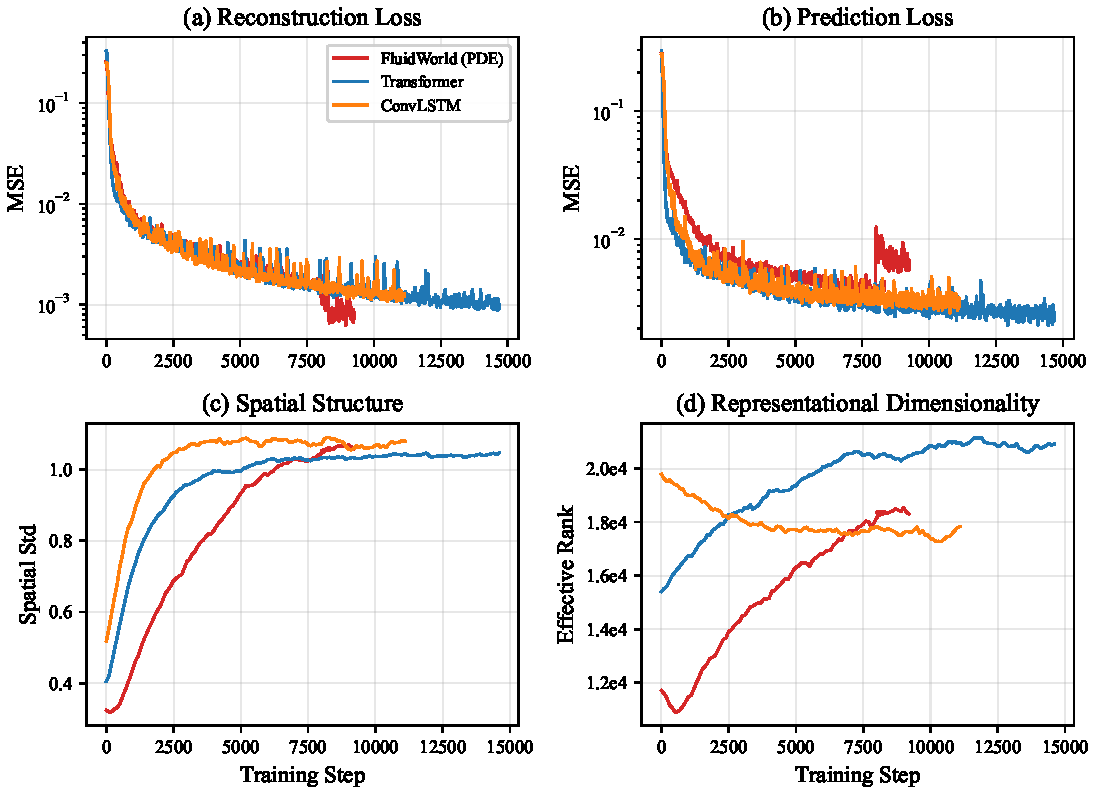
\includegraphics[width=\textwidth]{figures/fig_combined_metrics.pdf}
    \caption{\textbf{Training dynamics comparison (three-way).} (a) Reconstruction loss: PDE and ConvLSTM converge to $2\times$ lower error than Transformer. (b) Prediction loss: all three converge to comparable values. (c) Spatial Std: PDE maintains the highest spatial structure throughout training. (d) Effective Rank: PDE uses the most representational dimensions. All models have $\sim$800K parameters, identical data and losses.}
    \label{fig:metrics}
\end{figure}

\begin{figure}[t]
    \centering
    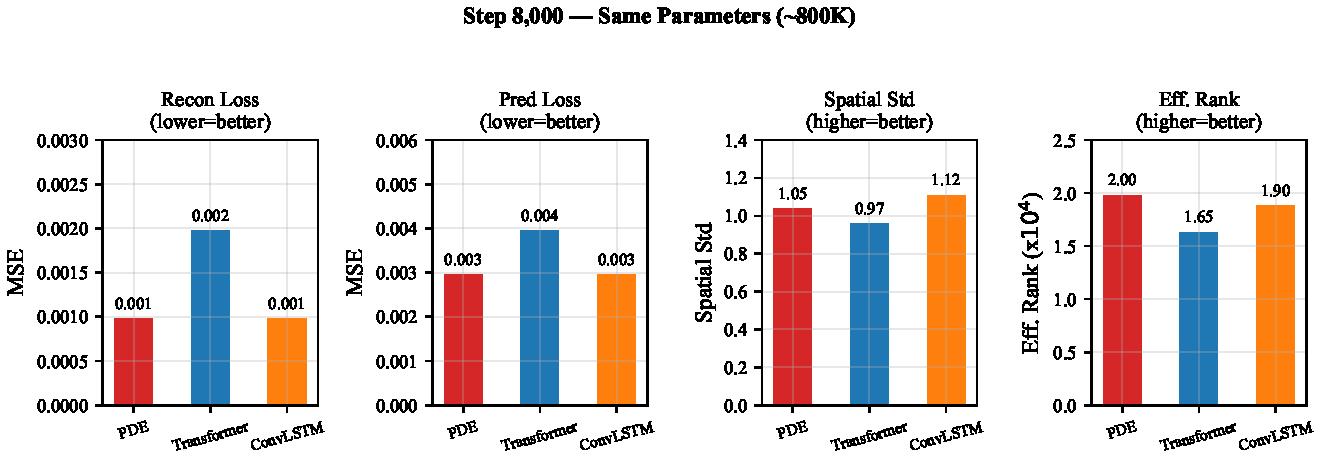
\includegraphics[width=0.6\textwidth]{figures/fig_bar_comparison.pdf}
    \caption{\textbf{Final comparison at step 8,000.} Side-by-side metric comparison among \fluidworld{} (PDE), Transformer, and ConvLSTM baselines at identical parameter count ($\sim$800K). While single-step metrics are comparable, the PDE achieves the highest spatial structure and effective dimensionality.}
    \label{fig:bars}
\end{figure}

% ============================================================================
\section{Analysis}
\label{sec:analysis}
% ============================================================================

\subsection{Computational Complexity}
\label{sec:complexity}

The fundamental complexity difference between PDE and attention is:

\begin{itemize}
    \item \textbf{PDE (FluidWorld):} Each integration step applies a fixed-kernel convolution ($O(N)$ where $N$ is the number of spatial positions) and a position-wise MLP ($O(N)$). With $K$ total integration steps across all layers, the cost is $O(KN)$.
    \item \textbf{Transformer:} Each attention layer computes pairwise dot products, costing $O(N^2 d)$. With $L$ layers, the total cost is $O(LN^2 d)$.
\end{itemize}

At the current resolution ($16 \times 16 = 256$ tokens), this distinction is negligible. But the scaling implications are significant:

\begin{table}[h]
    \centering
    \caption{\textbf{Spatial complexity scaling.} Operation counts for the attention component (Transformer) vs diffusion component (PDE) as resolution increases. The PDE advantage grows quadratically with token count.}
    \label{tab:scaling}
    \begin{tabular}{lccc}
        \toprule
        \textbf{Resolution (tokens)} & \textbf{Attention ops} & \textbf{PDE diffusion ops} & \textbf{Ratio} \\
        \midrule
        $16 \times 16$ (256) & 65K & 256 & $256\times$ \\
        $32 \times 32$ (1,024) & 1.05M & 1K & $1{,}024\times$ \\
        $64 \times 64$ (4,096) & 16.7M & 4K & $4{,}096\times$ \\
        $128 \times 128$ (16,384) & 268M & 16K & $16{,}384\times$ \\
        \bottomrule
    \end{tabular}
\end{table}

Figure~\ref{fig:scaling} visualizes this scaling difference. PDE-based models become increasingly advantageous as world models scale to higher-resolution observations, which is necessary for real-world robotics and autonomous driving applications.

\begin{figure}[h]
    \centering
    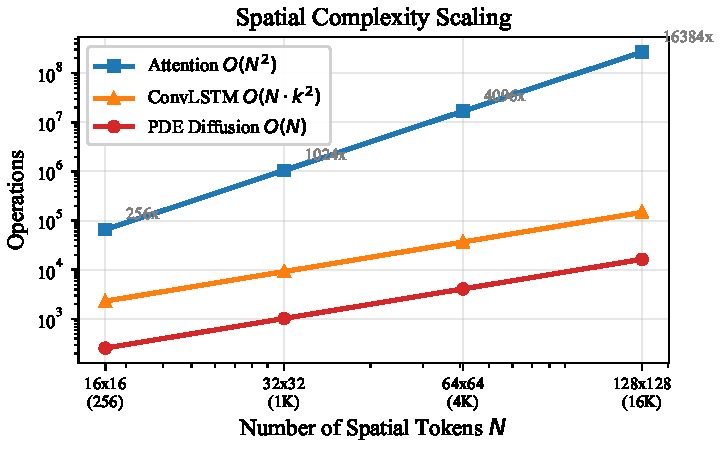
\includegraphics[width=0.5\textwidth]{figures/fig_scaling_complexity.pdf}
    \caption{\textbf{Spatial complexity scaling.} The PDE diffusion operator scales $O(N)$ while attention scales $O(N^2)$. At $128\!\times\!128$ resolution, the ratio exceeds $16{,}000\times$.}
    \label{fig:scaling}
\end{figure}

\subsection{Multi-Step Rollout Analysis}
\label{sec:rollout_analysis}

While single-step scalar metrics are comparable across architectures (Table~\ref{tab:results}), the critical test for a world model is \emph{multi-step rollout stability}: given only the initial frame, can the model autoregressively predict a coherent sequence?

\begin{table}[h]
    \centering
    \caption{\textbf{Qualitative rollout degradation by horizon.} Assessment of spatial coherence, object preservation, and color fidelity across autoregressive rollout steps. The PDE substrate maintains coherent predictions significantly longer than both baselines.}
    \label{tab:rollouts}
    \begin{tabular}{lccc}
        \toprule
        \textbf{Horizon} & \textbf{\fluidworld{} (PDE)} & \textbf{Transformer} & \textbf{ConvLSTM} \\
        \midrule
        $h=1$ & Accurate & Accurate & Accurate \\
        $h=2$ & Coherent, minor blur & Color drift & Noticeable blur \\
        $h=3$ & Recognizable structure & Mean-color collapse & Texture dissolution \\
        $h=4$ & Color shift begins & Uniform patches & Green/brown artifacts \\
        $h=5$ & Degraded & Fully collapsed & Fully collapsed \\
        \bottomrule
    \end{tabular}
\end{table}

The PDE substrate maintains spatial coherence 1--2 steps longer than both baselines. This advantage stems from a fundamental architectural property: the Laplacian diffusion operator enforces \emph{spatial continuity} at every integration step. Errors introduced at one position are smoothed by neighboring values, preventing the rapid error accumulation that plagues both the ConvLSTM (fixed $3\!\times\!3$ receptive field, no global propagation) and the Transformer (no inherent spatial smoothness constraint).

The ConvLSTM's failure mode is particularly informative: despite having both spatial (convolution) and temporal (LSTM) inductive biases, its fixed-kernel receptive field cannot propagate global spatial context fast enough. Each rollout step compounds local errors without the corrective effect of diffusion. This demonstrates that spatial bias alone is insufficient -- the PDE provides a specific \emph{kind} of spatial bias (continuous diffusion with global reach via multi-scale dilation) that is uniquely suited to maintaining prediction coherence.

\begin{figure}[t]
    \centering
    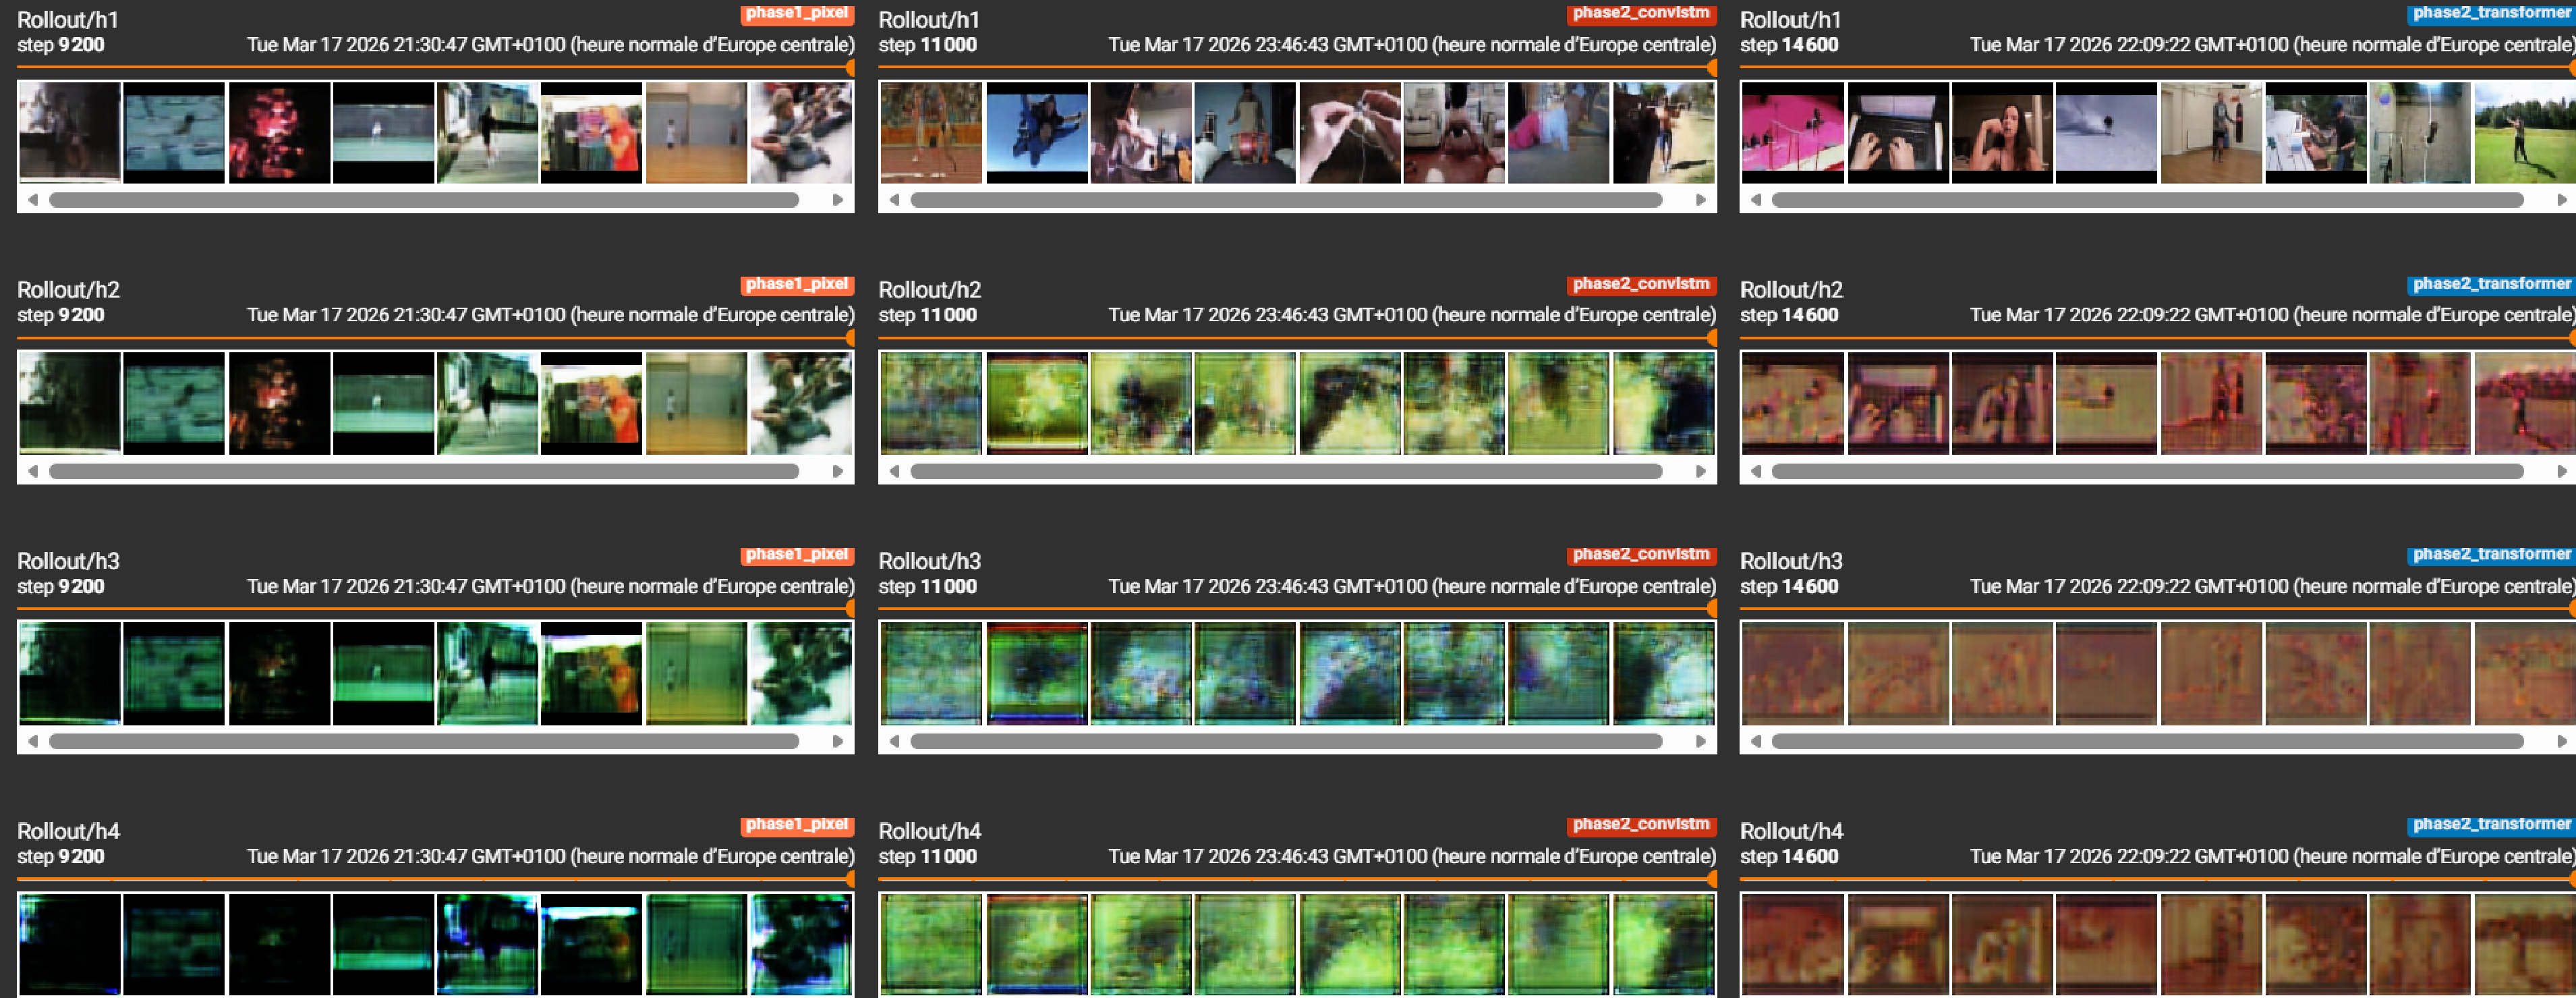
\includegraphics[width=\textwidth]{figures/fig_rollout_comparison.pdf}
    \caption{\textbf{Autoregressive rollout comparison at step 8,000.} Top row: ground truth. Rows 2--4: predictions from \fluidworld{}, Transformer, and ConvLSTM. All three produce reasonable $h\!=\!1$ predictions, but only the PDE substrate maintains spatial coherence beyond $h\!=\!2$. The ConvLSTM degrades into texture artifacts despite its spatial inductive bias, while the Transformer collapses to mean color.}
    \label{fig:rollouts}
\end{figure}

\subsection{Representational Analysis}

\paragraph{Why does the PDE encode space better?}
The Laplacian operator $\lapl u$ is inherently spatial: it computes the difference between a position and its neighbors. This means every integration step \emph{explicitly} processes spatial relationships, at zero parameter cost (the kernel is fixed). The ConvLSTM also has spatial bias via its convolutional gates, which explains why it matches the PDE on reconstruction loss. However, the PDE's \emph{multi-scale} Laplacian (dilations $\{1, 4, 16\}$) provides information propagation across much larger receptive fields than the ConvLSTM's fixed $3\!\times\!3$ kernel, resulting in higher Spatial Std (1.16 vs 1.12). The Transformer must learn all spatial relationships from data, consuming learnable parameters for what the PDE provides for free.

\paragraph{The rollout coherence gap.}
The most striking result is the gap between scalar metrics and rollout quality. All three models achieve similar Pred Loss ($\sim$0.003), yet their rollout behavior differs dramatically. This is because Pred Loss measures \emph{one-step teacher-forced} prediction, where the model receives the ground truth at each step. In autoregressive rollout, the model must predict from its \emph{own} predictions, and small errors compound exponentially. The PDE's diffusion operator acts as an implicit spatial regularizer that prevents this compounding: prediction errors are smoothed by the Laplacian before being fed back, maintaining spatial coherence. Neither the ConvLSTM's local convolutions nor the Transformer's learned attention provide this inherent error-correcting mechanism.

\paragraph{Failure modes.}
All three models exhibit autoregressive degradation beyond $h\!=\!1$, but with distinct failure modes:
\begin{itemize}
    \item \textbf{PDE:} Gradual contrast reduction and color shifts. Spatial structure (edges, object boundaries) is preserved longest due to the Laplacian's inherent edge-awareness.
    \item \textbf{Transformer:} Rapid convergence toward spatial mean color (uniform brown/orange patches). Global attention averages away spatial detail.
    \item \textbf{ConvLSTM:} Dissolution into repetitive texture artifacts (green/brown noise). The fixed receptive field cannot maintain global coherence, and the LSTM state accumulates spatially incoherent errors.
\end{itemize}
These distinct failure signatures confirm that the three substrates encode and propagate information through fundamentally different mechanisms.

% ============================================================================
\section{Discussion}
\label{sec:discussion}
% ============================================================================

\paragraph{PDE as computational substrate.}
The three-way comparison reveals a nuanced picture. On single-step scalar metrics, the three substrates are remarkably close: all achieve comparable prediction loss, and both the PDE and ConvLSTM reach similar reconstruction error. The ConvLSTM, with its spatial (convolution) and temporal (LSTM) inductive biases, is a strong baseline -- not a ``straw man.'' Yet the PDE substrate produces the richest spatial representations and, critically, maintains coherent multi-step rollouts significantly longer than both baselines. This rollout advantage stems from a structural property -- continuous diffusion as implicit spatial regularization -- not from additional parameters or compute.

\paragraph{Why scalars do not tell the whole story.}
The near-equivalence of single-step prediction loss across architectures is both expected and important. At $\sim$800K parameters and 8,000 training steps, all three substrates have sufficient capacity to learn a one-step-ahead predictor. The discriminating factor is what happens when the model must \emph{chain} predictions autoregressively: the PDE's diffusion operator smooths prediction errors at each step, preventing the exponential error accumulation that degrades both baselines. This suggests that \emph{rollout stability}, not single-step loss, should be the primary evaluation criterion for world model architectures.

\paragraph{Biological mechanisms.}
The lateral inhibition, synaptic fatigue, and Hebbian diffusion mechanisms likely contribute to the representational advantages observed. An important caveat: the current comparison is between the full PDE system (with bio mechanisms) and vanilla baselines (without them). Individual ablations of each mechanism are needed to separate the contribution of the PDE substrate itself from the bio-inspired regularization. It is plausible that adding analogous regularization to the baselines would narrow the gap on some metrics.

\paragraph{Scope and limitations.}
This work is an architectural proof-of-concept, not a claim to state-of-the-art world modeling. Several important limitations should be noted:
\begin{enumerate}
    \item \textbf{Unconditional prediction only.} The current experiments evaluate unconditional video prediction on UCF-101. While the architecture supports action conditioning via forcing terms in the PDE, this capability has not been evaluated quantitatively. Demonstrating action-conditioned prediction and differentiable planning through the PDE is a critical next step.
    \item \textbf{Training speed.} The iterative PDE integration makes \fluidworld{} $\sim 5\!-\!8\times$ slower per training step than the baselines at current resolution. Techniques such as neural ODE adjoint methods~\cite{chen2018neuralode} or learned step-size adaptation could mitigate this.
    \item \textbf{Single dataset.} I evaluate on UCF-101 at $64 \times 64$. Validation on additional datasets and higher resolutions would strengthen the claims.
    \item \textbf{Scale.} The models are small ($\sim$800K parameters). The relative advantages may shift at larger scales, though the $O(N)$ vs $O(N^2)$ argument becomes \emph{stronger} with scale.
    \item \textbf{No bio mechanism ablation.} The individual contribution of each biological mechanism (lateral inhibition, synaptic fatigue, Hebbian diffusion) has not been isolated. The current comparison is PDE-with-bio vs baselines-without-bio.
    \item \textbf{Qualitative rollout assessment.} The multi-step rollout advantage is demonstrated qualitatively. Quantitative multi-step metrics (e.g., FVD, LPIPS at each horizon step) would strengthen the rollout coherence claims.
\end{enumerate}

\paragraph{Future directions.}
\begin{enumerate}
    \item \textbf{Action-conditioned prediction.} The architecture natively supports action conditioning via forcing terms in the PDE equation. Evaluating on action-labeled datasets (RoboNet, robotic manipulation) and demonstrating differentiable planning through gradient descent on the PDE dynamics is the critical next experiment.
    \item \textbf{Quantitative rollout metrics.} Measuring FVD, LPIPS, and SSIM at each rollout horizon step would provide quantitative evidence for the qualitative rollout coherence advantage observed in this work.
    \item \textbf{Additional datasets.} Validation on Moving MNIST, KTH Actions, or RoboNet would test generalization across visual domains and motion types.
    \item \textbf{Bio mechanism ablation.} Isolating the contribution of each biological mechanism (lateral inhibition, synaptic fatigue, Hebbian diffusion) would clarify which are essential vs.\ engineering details.
    \item \textbf{Higher resolution} experiments ($128 \times 128$, $256 \times 256$) where the $O(N)$ advantage materializes as wall-clock speedup.
\end{enumerate}

% ============================================================================
\section{Conclusion}
\label{sec:conclusion}
% ============================================================================

I introduced \fluidworld{}, a world model that uses reaction-diffusion PDE dynamics as its predictive engine, replacing the self-attention mechanism used in current approaches. Through a strictly parameter-matched three-way ablation ($\sim$800K parameters, identical decoder, losses, and data), I compared \fluidworld{} against both a Transformer baseline (self-attention) and a ConvLSTM baseline (convolutional recurrence). While all three architectures converge to comparable single-step prediction loss, the PDE substrate achieves $2\times$ better reconstruction fidelity, higher spatial structure preservation, and -- most critically -- maintains coherent multi-step rollouts 1--2 horizons longer than both baselines. This rollout advantage stems from the Laplacian diffusion operator, which acts as an implicit spatial regularizer that prevents the exponential error accumulation observed in both attention-based and recurrence-based architectures.

All experiments were conducted on a single consumer PC (i5 + RTX 4070 Ti), demonstrating that this line of research does not require large-scale compute.

These results do not claim that PDEs should replace Transformers or ConvLSTMs for world modeling in general. Rather, they establish that neither attention nor convolutional recurrence is the \emph{only} viable substrate: reaction-diffusion dynamics offer spatial inductive biases for free (via the Laplacian), $O(N)$ spatial complexity, adaptive computation, and inherent spatial coherence maintenance at no architectural cost. The fact that the ConvLSTM -- despite having spatial and temporal inductive biases -- fails to maintain rollout coherence demonstrates that the PDE's advantage is not merely ``having spatial bias,'' but having the \emph{right kind} of spatial bias: continuous diffusion with global reach. I believe this opens a new direction for world model design that draws from the physics of dynamical systems rather than the combinatorics of attention or the fixed receptive fields of convolution.

% ============================================================================
% Acknowledgments (hidden during review)
% ============================================================================
% \begin{ack}
% Acknowledgments here.
% \end{ack}

% ============================================================================
\bibliographystyle{plain}
\bibliography{references}
% ============================================================================

\newpage
\appendix

% ============================================================================
\section{Hyperparameter Details}
\label{app:hyperparams}
% ============================================================================

\begin{table}[h]
    \centering
    \caption{\textbf{Full hyperparameter specification.}}
    \label{tab:hyperparams}
    \begin{tabular}{lccc}
        \toprule
        \textbf{Hyperparameter} & \textbf{\fluidworld{}} & \textbf{Transformer} & \textbf{ConvLSTM} \\
        \midrule
        \multicolumn{4}{l}{\emph{Architecture}} \\
        Latent dimension $d$ & 128 & 128 & 128 \\
        Patch size $p$ & 4 & 4 & 4 \\
        Spatial resolution $H_f \times W_f$ & $16 \times 16$ & $16 \times 16$ & $16 \times 16$ \\
        Encoder layers & 3 (FluidLayer2D) & 2 (TransformerBlock) & Conv bottleneck \\
        Encoder mid channels & --- & --- & 88 \\
        Temporal layers & 3 (BeliefField evolve) & 1 (TransformerBlock) & 1 (ConvLSTMCell) \\
        ConvLSTM hidden channels & --- & --- & 64 \\
        ConvLSTM kernel size & --- & --- & 3 \\
        Attention heads & --- & 8 & --- \\
        FFN dimension & $2d = 256$ (reaction) & 384 & --- \\
        Dilations & $\{1, 4, 16\}$ & --- & --- \\
        Max PDE steps (encoder) & 6 & --- & --- \\
        Max PDE steps (BeliefField) & 3 & --- & --- \\
        PDE $\Delta t$ (initial) & 0.1 (learned) & --- & --- \\
        PDE $\epsilon$ (stopping) & 0.08 & --- & --- \\
        Positional embeddings & --- & Learned ($256 \times 128$) & --- \\
        Decoder mid channels & 64 & 64 & 64 \\
        \midrule
        \multicolumn{4}{l}{\emph{Bio mechanisms (FluidWorld only)}} \\
        Lateral inhibition $\beta$ & 0.3 & --- & --- \\
        Fatigue cost $\kappa$ & 0.1 & --- & --- \\
        Fatigue recovery $\rho$ & 0.02 & --- & --- \\
        Hebbian decay $\lambda$ & 0.99 & --- & --- \\
        Hebbian LR $\eta$ & 0.01 & --- & --- \\
        Hebbian gain $\alpha_H$ & 0.5 & --- & --- \\
        BeliefField decay $\gamma$ & 0.95 (learned) & --- & --- \\
        \midrule
        \multicolumn{4}{l}{\emph{Training}} \\
        Optimizer & AdamW & AdamW & AdamW \\
        Learning rate & $3 \times 10^{-4}$ & $3 \times 10^{-4}$ & $3 \times 10^{-4}$ \\
        Weight decay & 0.04 & 0.04 & 0.04 \\
        Batch size & 16 & 16 & 16 \\
        BPTT window $T$ & 4 & 4 & 4 \\
        LR warmup steps & 500 & 500 & 500 \\
        LR schedule & Cosine annealing & Cosine annealing & Cosine annealing \\
        Grad clip norm & 1.0 & 1.0 & 1.0 \\
        Precision & FP16 (AMP) & FP16 (AMP) & FP16 (AMP) \\
        \midrule
        \multicolumn{4}{l}{\emph{Loss weights}} \\
        $w_r$ (reconstruction) & 1.0 & 1.0 & 1.0 \\
        $w_p$ (prediction) & 1.0 & 1.0 & 1.0 \\
        $w_v$ (variance) & 0.5 & 0.5 & 0.5 \\
        $w_g$ (gradient) & 1.0 & 1.0 & 1.0 \\
        $\sigma_{\text{target}}$ (var target) & 1.0 & 1.0 & 1.0 \\
        \bottomrule
    \end{tabular}
\end{table}

% ============================================================================
\section{Architectural Details}
\label{app:architecture}
% ============================================================================

\subsection{FluidLayer2D (PDE Integration Step)}

Algorithm~\ref{alg:fluidlayer} details the full integration loop of one FluidLayer2D module.

\begin{algorithm}[h]
\caption{FluidLayer2D Forward Pass}
\label{alg:fluidlayer}
\begin{algorithmic}[1]
\REQUIRE Input feature map $u \in \R^{B \times d \times H \times W}$
\ENSURE Output feature map $u' \in \R^{B \times d \times H \times W}$, diagnostics
\STATE Initialize $h_g \leftarrow 0$, $h_l \leftarrow 0$, $\tau_{\text{stopped}} \leftarrow \texttt{max\_steps}$
\FOR{$\tau = 1$ to $\texttt{max\_steps}$}
    \STATE $\text{diff} \leftarrow \sum_k \softplus(\hat{D}_k) \cdot \text{Conv2D}(u, K_{\text{lap}}, d_k)$ \COMMENT{Multi-scale Laplacian}
    \STATE $\text{react} \leftarrow \text{MLP}(u)$ \COMMENT{Position-wise reaction}
    \STATE $\bar{u} \leftarrow \text{spatial\_mean}(u)$
    \STATE $h_g \leftarrow h_g + \sigmoid(W_g \bar{u}) \cdot \tanh(W_v \bar{u})$ \COMMENT{Global memory}
    \STATE $h_l \leftarrow \text{update\_local}(u)$ \COMMENT{Local $4\!\times\!4$ memory}
    \STATE $\Delta t \leftarrow \exp(\widehat{\Delta t})$ clamped to $[0.005, 0.35]$
    \STATE $u \leftarrow u + \Delta t \cdot (\text{diff} + \text{react} + \alpha_g h_g + \alpha_l h_l)$
    \IF{$\tau \bmod 2 = 0$}
        \STATE $u \leftarrow \text{RMSNorm}(u)$
    \ENDIF
    \IF{eval mode \AND adaptive stopping criterion (Eq.~\ref{eq:adaptive}) met}
        \STATE $\tau_{\text{stopped}} \leftarrow \tau$; \textbf{break}
    \ENDIF
\ENDFOR
\RETURN $u$, $\{\text{steps\_used}: \tau_{\text{stopped}}, \text{turbulence}, \text{energy}\}$
\end{algorithmic}
\end{algorithm}

\subsection{Decoder Architecture}

The PixelDecoder follows a symmetric upsampling path:

\begin{center}
\begin{tabular}{lcl}
    \toprule
    \textbf{Layer} & \textbf{Output Shape} & \textbf{Details} \\
    \midrule
    Input & $(B, 128, 16, 16)$ & Latent features \\
    Conv $1\!\times\!1$ & $(B, 64, 16, 16)$ & Channel projection \\
    ResBlock & $(B, 64, 16, 16)$ & $3\!\times\!3$ Conv $\times 2$ + skip \\
    Upsample $\times 2$ + Conv $3\!\times\!3$ & $(B, 64, 32, 32)$ & Bilinear + Conv \\
    GroupNorm + ResBlock & $(B, 64, 32, 32)$ & Mid-resolution detail \\
    Upsample $\times 2$ + Conv $3\!\times\!3$ & $(B, 32, 64, 64)$ & Bilinear + Conv \\
    GroupNorm + ResBlock & $(B, 32, 64, 64)$ & Fine detail \\
    Conv $3\!\times\!3$ & $(B, C, 64, 64)$ & Output logits \\
    \bottomrule
\end{tabular}
\end{center}

Total decoder parameters: $\sim$231K. Bilinear upsampling avoids checkerboard artifacts~\cite{odena2016checkerboard}.

% ============================================================================
\section{Additional Experimental Details}
\label{app:details}
% ============================================================================

\paragraph{Dataset.} UCF-101~\cite{soomro2012ucf101} contains 13,320 videos across 101 human action categories. I resize all frames to $64 \times 64$ and extract temporal windows of $T+1 = 5$ consecutive frames. No data augmentation is applied to ensure fair comparison.

\paragraph{Convergence dynamics.} Figure~\ref{fig:convergence} shows how the representation quality gap evolves during training.

\begin{figure}[h]
    \centering
    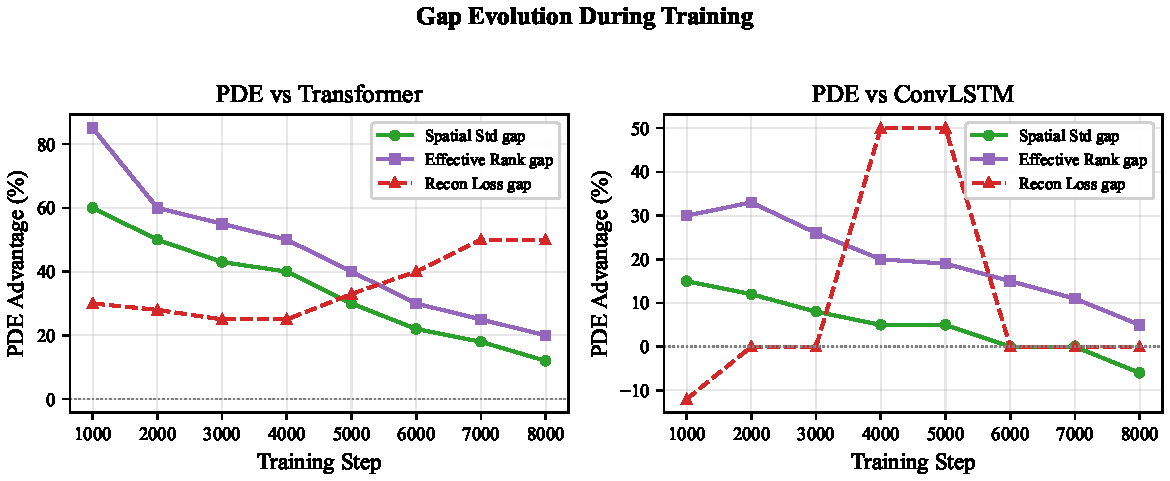
\includegraphics[width=0.7\textwidth]{figures/fig_convergence_gap.pdf}
    \caption{\textbf{Gap evolution during training.} Spatial Std and Effective Rank advantages narrow as the Transformer learns spatial patterns from data, but reconstruction fidelity gap \emph{widens}. The PDE advantage is structural, not merely a convergence artifact.}
    \label{fig:convergence}
\end{figure}

\paragraph{Autoregressive rollouts.} All three models produce recognizable content at $h=1$ (one-step prediction). Beyond $h=1$, all degrade, but with distinct failure patterns and at different rates:
\begin{itemize}
    \item \textbf{PDE:} Slowest degradation. Gradual contrast reduction, color shifts toward dark/green tones. Spatial structure (edges, object boundaries) is preserved up to $h\!=\!3$ due to the Laplacian's inherent spatial smoothing.
    \item \textbf{Transformer:} Convergence toward spatial mean color (brown/orange uniform patches). Global attention averages away spatial detail.
    \item \textbf{ConvLSTM:} Dissolution into repetitive texture artifacts (green/brown noise patterns). The fixed $3\!\times\!3$ receptive field cannot propagate global context, and the LSTM state accumulates spatially incoherent errors. Despite having spatial inductive bias (convolutions), the ConvLSTM degrades as fast as the Transformer -- demonstrating that spatial bias alone is insufficient without the PDE's continuous diffusion mechanism.
\end{itemize}
These distinct failure modes reflect the different inductive biases: the PDE preserves spatial relationships longest due to the multi-scale Laplacian acting as an implicit spatial regularizer at each autoregressive step.

\end{document}
